
\de{ĐỀ THI HỌC KỲ I NĂM HỌC 2022-2023}{THPT Nguyễn Thị Diệu}




%%==========Bài 1
\begin{bt}%[1,0 điểm]%[0D1B3-4]%[Dự án đề kiểm tra HK1 NH22-23-Don Lee]%[THPT Nguyễn Thị Diệu]
	Cho hai tập hợp $A=(-2; 5]$, $B=(1;+\infty)$. Xác định các tập hợp $A\cap B$, $A\cup B$, $A\backslash B$, $C_{\mathbb{R}}B$.
	%\dapso{$A \cap B=\left(1;5\right] $, $A \cup B=(-2;+\infty)$, $A \backslash B=(-2;1]$, $ C_{\mathbb{R}} B=(-\infty;1]$.}
	\loigiai{
		Ta có $A\cap B=\left(1;5\right]$, $A\cup B=(-2;+\infty)$, $A\backslash B=(-2;1]$, $C_{\mathbb{R}}B=(-\infty;1]$.
	}
\end{bt}

%%==========Bài 2
\begin{bt}[1,0 điểm]%[0D3B1-2]%[Dự án đề kiểm tra HK1 NH22-23-Don Lee]%[THPT Nguyễn Thị Diệu]
	Tìm tập xác định của hàm số $y=\dfrac{\sqrt{x-2}}{3x^{2}-10x+3}$.
	%\dapso{$\mathscr{D}=[2;+\infty)\setminus\{3\}$.}
	\loigiai{
		Điều kiện xác định $\heva{&x-2\ge 0\\&3x^{2}-10x+3\ne 0} \Leftrightarrow \heva{&x\ge 2\\&x\ne \dfrac{1}{3}\,\,\text{và}\,\, x\ne 3} \Leftrightarrow \heva{&x\le 2\\&x\ne 3.}$\\
		Tập xác định của hàm số $\mathscr{D}=[2;+\infty)\setminus\{3\}$.
	}
\end{bt}

%%==========Bài 3
\begin{bt}%[2,5 điểm]%[0D3B2-2]%[0D3B2-1]%[0D3B2-4]%[Dự án đề kiểm tra HK1 NH22-23-Don Lee]%[THPT Nguyễn Thị Diệu]
	\begin{enumerate}
		\item Xác định các hệ số $a$, $b$ của parabol $(P)\colon y=ax^{2}+bx+2$, biết rằng $(P)$ qua $A(3;-1)$ và có trục đối xứng là đường thẳng $x=1$.
		\item Lập bảng biến thiên và vẽ đồ thị hàm số $y=-x^{2}+2x+2$.
		\item Tìm tọa độ giao điểm của đường thẳng $d\colon y=5x-2$ và parabol $(P)\colon y=-x^{2}+2x+2$.
	\end{enumerate}
	%\dapso{a) $a=-1$; $b=2$; c) $(1;3)$, $(-4;-22)$.}
	\loigiai{
		\begin{enumerate}
			\item Do $(P)\colon y=ax^{2}+bx+2$ qua $A(3;-1)$ và có trục đối xứng là đường thẳng $x=1$ nên ta có
				\[\heva{&a\cdot 3^2+b\cdot 3+2=-1\\&-\dfrac{b}{2a}=1} \Leftrightarrow \heva{&a=-1\\&b=2.}\]
				Vậy $(P)\colon y=-x^{2}+2x+2$.
			\item Bảng biến thiên và vẽ đồ thị hàm số $y=-x^{2}+2x+2$
				\begin{center}
					
\begin{tikzpicture}[>=stealth]
						\tkzTabInit[nocadre=false,lgt=1,espcl=2,deltacl=0.5]{$x$/.7 ,$y$/2}
						{$-\infty$ , $1$ , $+\infty$}
						\tkzTabVar{-/$-\infty$ , +/$3$ , -/$-\infty$}
					\end{tikzpicture}
				\end{center}
			\item Tọa độ giao điểm của đường thẳng $d\colon y=5x-2$ và parabol $(P)\colon y=-x^{2}+2x+2$ là nghiệm của phương trình $-x^{2}+2x+2=5x-2$. $(1)$\\
				Ta có $(1) \Leftrightarrow -x^{2}-3x+4=0 \Leftrightarrow x=-4; x=1$.\\
				Vậy tọa độ giao điểm của đường thẳng $d\colon y=5x-2$ và parabol $(P)\colon y=-x^{2}+2x+2$ là $M(-4; -22)$ và $N(1; 3)$.
		\end{enumerate}
	}
\end{bt}

%%==========Bài 4
\begin{bt}%[1,0 điểm]%[0D2B2-3]%[Dự án đề kiểm tra HK1 NH22-23-Don Lee]%[THPT Nguyễn Thị Diệu]
	Tính giá trị nhỏ nhất của biểu thức $F(x; y)=12x-15y$ với $(x; y)$ thỏa mãn hệ bất phương trình $\heva{&x+3y+3\geq 0\\&x-2y+3\geq 0\\&x+y-3\leq 0.}$
	%{Giá trị nhỏ nhất $F(-3;0)=-36$.}
	\loigiai{
		\immini
		{\begin{itemize}
			\item Vẽ ba đường thẳng $y=-\dfrac{1}{3}x-1$; $y=\dfrac{1}{2}x+\dfrac{3}{2}$ và $y=-x+3$.
			\item Miền nghiệm thỏa mãn hệ bất phương trình $\heva{&x+3y+3\geq 0\\&x-2y+3\geq 0\\&x+y-3\leq 0}$ là miền trong của tam giác $ABC$ kể cả biên.
			\item Ta có $F(-3;0)=-36$; $F(1; 2)=-18$; $F(6; -3)=117$. Vậy $\min F(x; y)=F(-3;0)=-36$.
		\end{itemize}}
		{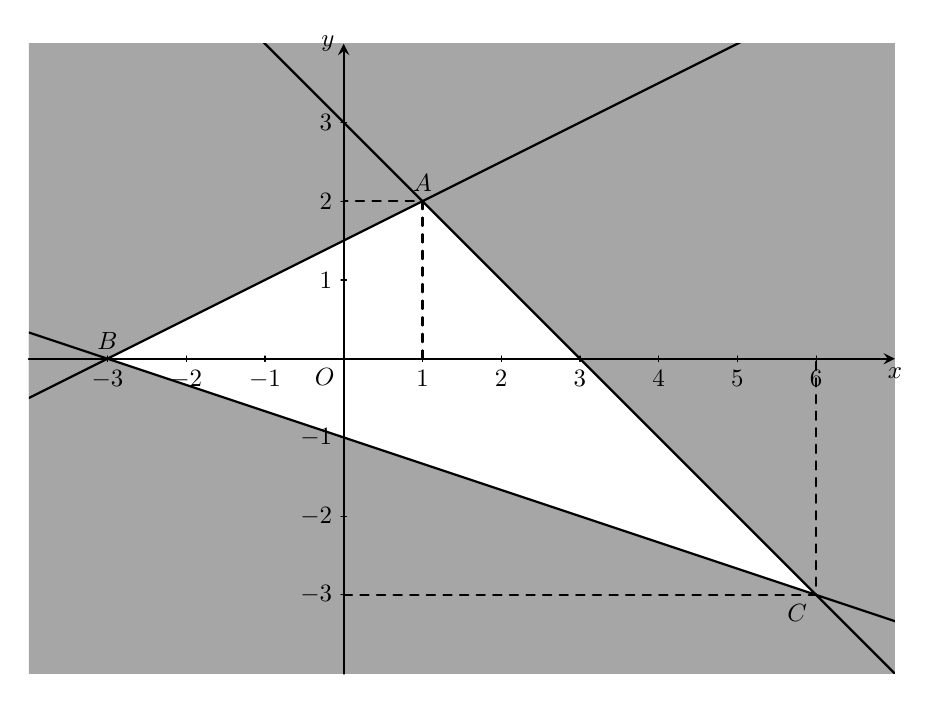
\begin{tikzpicture}[line join=round, line cap=round,>=stealth,thick]
					\tikzset{every node/.style={scale=0.9}}
					\begin{scope}
						\clip (-4,-4) rectangle (7,4);
						\fill[black!35] (-22,6.33)--(-22,-6.33)--(16,-6.33)--cycle;
						\fill[black!35] (-16,-6.5)--(-16,6.5)--(10,6.5)--cycle;
						\fill[black!35] (-7,10)--(10,10)--(10,-7)--cycle;
						\draw (-21,6)--(15,-6)  (9,6)--(-15,-6)  (-3,6)--(9,-6);
						%\draw (-3,6)--(9,-6) node [pos=0.45, above, sloped] {$x+y-3=0$};
					\end{scope}
					\draw[->] (-4,0)--(7,0) node[below]{$x$};
					\draw[->] (0,-4)--(0,4) node[left]{$y$};
					\draw (0,0) node[below left]{$O$};
					\draw (1,2) node[above]{$A$};
					\draw (-3,0) node[above]{$B$};
					\draw (6,-3) node[below left]{$C$};
					%\draw (4,3) node[pos=0.45, below right, sloped]{$x-2y+3=0$};
					%\draw (1,-2) node[pos=0.45, below left, sloped]{$x+3y+3=0$};
					%\draw (6,-3) node[below left]{$C$};
					\draw[dashed] (1,0)--(1,2)--(0,2)  (0,-3)--(6,-3)--(6,0);
					\foreach \x in {-3,-2,-1,1,2,3,4,5,6}
					\draw[thin] (\x,1pt)--(\x,-1pt) node [below] {$\x$};
					\foreach \y in {-3,-2,-1,1,2,3}
					\draw[thin] (1pt,\y)--(-1pt,\y) node [left] {$\y$};
		\end{tikzpicture}}
	}
\end{bt}
%%==========Bài 5
\begin{bt}%[0T4B3-1]%[Dự án đề kiểm tra HKII NH22-23- Phan Trung Hiếu]%[THPT Nguyên Thị Diệu]
	Cho tam giác $A B C$ có $A B=8$, $A C=5$, $ \widehat{B A C}=40^{\circ}$. Tính độ dài cạnh $B C$, bán kính đường tròn ngoại tiếp, diện tích và độ dài đường cao $A H$ của tam giác $ABC$. (Kết quả làm tròn đến hàng phần trăm)
	\dapso{$BC=5{,}26$; $R=4{,}1$; $S=12{,}86$; $AH=4{,}88$.}
	\loigiai{
		Độ dài cạnh $BC$ là
		\begin{equation*}
			BC=\sqrt{AB^2+AC^2-2\cdot AB\cdot AC\cdot\cos(\widehat{BAC})} =\sqrt{ 8^2+5^2-2\cdot8\cdot5\cdot\cos40^\circ}\approx5{,}26.
		\end{equation*}
		Diện tích tam giác $ABC$ là
		\begin{equation*}
			S = \dfrac{1}{2}\cdot AB\cdot AC\cdot\sin40^\circ = \dfrac{1}{2}\cdot8\cdot5\cdot\sin40^\circ \approx12{,}86.
		\end{equation*}
		Bán kính đường tròn ngoại tiếp tam giác $ABC$ là
		\begin{equation*}
			R = \dfrac{AB\cdot AC\cdot BC}{4S}=\dfrac{8\cdot5\cdot5{,26}}{4\cdot12{,}86}\approx 4{,}1.
		\end{equation*}
		Đường cao $AH$ của tam giác $ABC$ là
		\begin{equation*}
			AH = \dfrac{2S}{BC}=\dfrac{2\cdot12{,}86}{5{,}26}\approx4{,88}.
		\end{equation*}
	}
\end{bt}

%%==========Bài 6
\begin{bt}%[0T5G2-2]%[Dự án đề kiểm tra HKII NH22-23- Phan Trung Hiếu]%[THPT Nguyên Thị Diệu]
	Cho hình bình hành $A B C D$ có tâm $O$.
	\begin{enumerate}
		\item Với $M$ là điểm tùy ý, chứng minh rằng $\vv{M A}+\vv{M B}+\vv{M C}+\vv{M D}=4 \vv{M O}$.
		\item Gọi $I$, $J$ lần lượt là điểm trên các đoạn $B C, B D$ sao cho $\vv{B C}+5 \vv{I B}=\vv{0}$, $ 2 \vv{JB}+\vv{J O}=\vv{0}$. Chứng minh rằng ba điểm $A$, $I$, $J$ thẳng hàng.
	\end{enumerate}
	\loigiai{
		\begin{center}
			\begin{tikzpicture}[thick]
				\path
				(2,2) coordinate (A)
				(0,0) coordinate (B)
				(5,0) coordinate (C)
				($(A)!.5!(C)$) coordinate (O)
	 			($(A)+(C)-(B)$) coordinate (D)
	 			($(B)!.2!(C)$) coordinate (I)
	 			($(B)!1/3!(O)$) coordinate (J)
	 			;
	 			\draw (A)--(B)--(C)--(D)--cycle (B)--(D) (A)--(C);
	 			\draw[dashed,red] (A)--(J)--(I);
	 			\foreach \x/\g in {A/90,B/180,C/-45,D/90,I/-90,O/90,J/90}
				\fill[black] 	(\x) circle (1pt)
				($(\g:3mm)+(\x)$) node {$\x$};
			\end{tikzpicture}
		\end{center}
		\begin{enumerate}
			\item $O$ là giao điểm 2 đường chéo của hình bình hành $ABCD$ nên $O$ là trung điểm của $AC$ và $BD$ nên ta có
			\begin{equation*}
				\vv{OA}+\vv{OC} = \vv{0}\quad\text{và}\quad\vv{OB}+\vv{OD}=\vv{0}.
			\end{equation*}
			Ta có
			\begin{equation*}
				\vv{M A}+\vv{M B}+\vv{M C}+\vv{M D}=4\vv{MO}+(\vv{OA}+\vv{OC})+(\vv{OB}+\vv{OD})=4\vv{MO}.
			\end{equation*}
			\item Ta có
			\begin{equation*}
				2\vv{AB}+\vv{AO} = 2\vv{JB}+\vv{JO}+3\vv{AJ}=3\vv{AJ}.
			\end{equation*}
			Suy ra
			\begin{equation*}
				\vv{AJ}=\dfrac{2}{3}\vv{AB}+\dfrac{1}{3}\vv{AO}=\dfrac{2}{3}\vv{AB}+\dfrac{1}{6}\vv{AC},
			\end{equation*}
			hay
			\begin{equation}\label{1}
				6\vv{AJ}=4\vv{AB}+\vv{AC}.
			\end{equation}
			Vì $\vv{BC}+5\vv{IB}=\vv{0}$ nên $I$ nằm giữa $B$ và $C$ và $\vv{BC}=\dfrac{5}{4}\vv{IC}$. Suy ra $\dfrac{1}{4}\vv{IC}+\vv{IB}= \vv{0}$.\\
			Mặt khác
			\begin{equation*}
				\vv{AB}+\dfrac{1}{4}\vv{AC}=\vv{IB}+\dfrac{1}{4}\vv{IC}+\dfrac{5}{4}\vv{AI}
			\end{equation*}
			Suy ra,
			\begin{equation}\label{2}
				5\vv{AI} = 4\vv{AB}+\vv{AC}.
			\end{equation}
			Từ (\ref{1}) và (\ref{2}), ta có $6\vv{AJ}=5\vv{AI}$ hay $\vv{AI}=\dfrac{6}{5}\vv{AJ}$.\\
			Vậy $A$, $I$, $J$ thẳng hàng.
		\end{enumerate}
	}
\end{bt}

%%==========Bài 7
\begin{bt}%[0T6B3-4]%[Dự án đề kiểm tra HKII NH22-23- Phan Trung Hiếu]%[THPT Nguyên Thị Diệu]
	Một cảnh sát giao thông ghi lại tốc độ (đơn vị: $\mathrm{km} / \mathrm{h}$) của $25$ xe qua trạm như sau:
	\begin{center}
		\begin{tabular}{|l|l|l|l|l|l|l|l|l|l|l|l|l|}
			\hline
			$40$ & $35$ & $50$ & $60$ & $55$ & $35$ & $60$ & $45$ & $60$ & $50$ & $55$ & $50$ & $40$ \\
			\hline
			$45$ & $45$ & $40$ & $50$ & $60$ & $45$ & $35$ & $55$ & $45$ & $60$ & $45$ & $45$ &  \\
			\hline
		\end{tabular}
	\end{center}
	\begin{enumerate}
		\item Lập bảng phân bố tần số và xác định số trung vị, mốt của bảng số liệu trên.
		\item Tính tốc độ trung bình của $25$ xe qua trạm.
	\end{enumerate}
	\dapso{a) $Q_2=45$, $M_o=45$; b) $\overline{x}=48{,}2$.}
	\loigiai{
		\begin{enumerate}
			\item Bảng phân bố tần số
			\begin{center}
				\begin{tabular}{|c|c|c|c|c|c|c|c|}
					\hline
					Tốc độ&$35$&$40$&$45$&$50$&$55$&$60$& $N$\\
					\hline
					Tần số&$3$&$3$&$7$&$4$&$3$&$5$&$25$\\
					\hline
				\end{tabular}
			\end{center}
			Mốt của bảng số liệu là $M_0=45$.\\
			Trung vị của mẫu số liệu là $Q_2=45$.
			\item Tốc độ trung bình của 25 xe qua trạm là
			\begin{equation*}
				\overline{x}=\dfrac{35\cdot3+40\cdot3+45\cdot7+50\cdot4+55\cdot3+60\cdot5}{25}=48{,}2.
			\end{equation*}
		\end{enumerate}
	}
\end{bt}
